\documentclass{article}

\usepackage[utf8]{inputenc}
% Use nameref to cite supporting information files (see Supporting Information section for more info)
\usepackage{nameref,hyperref}
% amsmath and amssymb packages, useful for mathematical formulas and symbols
\usepackage{amsmath,amssymb}
% useful for consistent display and control of units of measurement
\usepackage{siunitx}
% figures!
\usepackage{graphicx}
% for including TODO notes
\usepackage{todonotes}
% snyntax highlighting for code
\usepackage{minted}

\title{Measurement and Analysis of Equivalent Fall Height of Ski and Snowboard Jumps with Explanation Through Case Studies}
\author{Bryn Cloud, Mont Hubbard, Christopher Brown, Jason K. Moore}
\date{\today}

\begin{document}

\maketitle

\section*{Outline}
%
\begin{itemize}
  \item Intro
  \begin{itemize}
    \item history
    \item moral imperative - engineers obligation to the public
    \item summary of paper
  \end{itemize}
  \item EFH meaning and importance
  \begin{itemize}
    \item Safe slope equation: EFH-y(x) equivalence
    \item design - find y(x) for given EFH
    \item analysis: find EFH given y(x)
  \end{itemize}
  \item Online access of skijumpdesign.info
  \begin{itemize}
    \item does both design and analysis
    \item free and easy
    \item open source
    \item interleaves with ASTM measurements of jump shapes (Excel files etc.)
  \end{itemize}
  \item Measurement of jump shape
  \begin{itemize}
    \item using DGPS
    \item 1 cm accuracy
    \item as remote as 1 Km
    \item rover receiver on skier allow versatility
  \end{itemize}
  \item Actual examples of design and analysis and measurement
  \begin{itemize}
    \item Salvini
    \item Sierra-Tahoe??
    \item Knoernschild
  \end{itemize}
  \item Conclusions and recommendations
\end{itemize}

\begin{abstract}
    TODO
\end{abstract}

\section{Introduction}
%
Greater human-object impact velocity normal to the impact surface causes
greater injuries\todo{We need strong citations for this claim.}.
A common surrogate for measures impact velocity is ``equivalent fall height''.
Equivalent fall height provides a conceptually simple interpretation of the
danger from impact.
The equivalent fall height of ski and snowboard jumps can be calculated if the
Cartesian coordinates of the cross-sectional profile at the jumper's path
center line and takeoff angle are available.
Reduction in the equivalent fall height is one of several design factors that
can reduce injury.

This paper 1) explains why equivalent fall height is important to assess in
jump design, 2) explains how to measure the Cartesian coordinates of a jump, 3)
shows how to calculate equivalent fall height, 3) details a user-friendly web
application for calculating equivalent fall height, and 4) uses some cases
studies to show how dangerous past constructed jumps can be.

\subsection{History}
%
\todo[inline]{Mont should write this section.}

\subsection{Moral Imperative}
%
Reducing the risk of injuries on manufactured jumps motivates this work.
Intelligent, engineering design based on classical mechanics shapes features to
limit EFH. This complies with the first canon of engineering ethics ``Hold
paramount the safety, health and welfare of the public''. In the context of
snow sport safety, the first canon compels engineers to direct their technical
expertise to protecting snow sport participants from injuries.

People unfamiliar with the legal and insurance systems in the United States
might fail to appreciate that technical literature is corrupted in the defense
of unsafe practices and corporate profits. Peer-reviewed, technical literature
provides support for testimony in U.S. lawsuits. Plaintiffs and defendants both
hire their own experts to testify. Authors of technical papers can make money
by testifying. When it is for the defense, this testimony can result in denying
compensation to injuries, and serves to prolong unsafe practices in snowsports.
Rarely do experts report any conflicts of interest in their papers and
presentations, or when they organize and chair meetings or edit publications.
Financial support for publications used by expert witnesses can be routed
through consulting companies to pretend some deniability of conflicts in their
papers.

Designing jumps to limit EFH and reduce the risk of injuries is based on
well-known and well-established laws of mechanics. The concept that designing
jumps to limit EFH and control energy dissipation rates can reduce the risk is
irrefutable. It is basic physics. To counter this solid, fundamental,
scientific concept for defense experts, confounding factors are introduced.
These serve to cloud and confuse the basic issues. Consider three examples of
papers co-authored by well-known defense experts who testify for the ski
industry in ski injury cases. \cite{Shealy2010} conducted a study of the
influence of take-off speeds on landing locations with a series of jumpers who
appeared to use the feature and show that the people who jumped while they were
measuring land within a narrow region. \cite{Shealy2015} total serious
injury rates appear not to have changed while of terrain parks increased. In an
article on landing positions \cite{Scher2015} show that body orientation at
impact is important. The first two studies do a poor job of isolating
variables, and were not intended to, and the third suffers from restriction of
range. None of these papers are intended to reduce injury rates. No ways are
suggested in which their findings could be used to promote the safety, health
and welfare of the public.

Testifying for an injured plaintiff, or to defend corporations, in injury
cases, are not equivalent actions ethically, neither is authoring apparently
all kinds of conflicting papers on injuries. The former attempts to address in
problems that cause injuries, holding paramount the safety health and welfare
of the public. The latter attempts to defend the practices that might have
contributed to the injury to limit financial losses of insurance companies.
Proverbial two sides to every question do not exist in science and engineering.
Experiments in snowsports, no matter how expensive and sophisticated the
instrumentation, are not going to disprove the fundamental laws of classical
mechanics. If some statics or experimental results do not seem to support work
based on classical mechanics, then there is a problem with the statistical or
experimental design or their interpretation, and not with classical mechanics.
Defending practices that lead to injuries at the service of industry can
prolong these practices, which can lead to further injuries, clearly violating
the first canon of engineering ethics.

\section{Equivalent Fall Height}
%
The equivalent fall height $h$ of an object is defined as
%
\begin{align}
  h = \frac{v^2}{2g}
  \label{eq:efh_general}
\end{align}
%
where $v$ is the impact velocity of an object and $g$ is the acceleration due
to gravity. This definition results from equating the kinetic energy of an
object moving at velocity $v$ with the potential energy of the same object at a
height $h$ above the ground. Equivalent fall height is commonly used to measure
impact severity by OSHA, FAA, and others~\cite{Hubbard2012}. To calculate the
equivalent fall height when impact is at an angle from the impact surface, the
equation becomes
%
\begin{align}
  h = v_{\perp}^2/2g
  \label{eq:efh_slope}
\end{align}
%
where $v_{\perp}$ is the velocity perpendicular to the impact surface. To
calculate the equivalent fall height of a ski slope, we have defined the
Cartesian coordinates of jump cross section in the jumper's path. We select the
takeoff point to be the origin, as it is a common feature of all jumps.
For the jumper to have a low impact velocity, and thus small equivalent fall
height, there must only be a small misalignment between the takeoff\todo{Should
this be landing angle? Or is this referring to the case of a flat surface?}
angle, $\theta$, and the slope angle, $\phi$.
%
\begin{align}
  v_{\perp} = \sqrt{2gh} = v\sin(\theta - \phi)
\end{align}

If no aerodynamic forces is assumed, the projectile equations show that x, y
system is linear and quadratic in time.\todo{Not sure what this sentence is
supposed to mean}.
Inverting the parabola gives the initial velocity, $v_o$ required to reach a
given location:
%
\begin{align}
  v_o = \sqrt{\frac{x^2g}{2(x \tan \theta_o -y)\cos^{2}\theta}}
\end{align}

Using the above equations, the equivalent fall height h is a function of only
four variables: takeoff angle $\theta$, landing coordinates $(x, y)$, and the slope of
the landing surface $\frac{dy}{dx}$ also written as $\tan\phi$. Given a takeoff
angle, one can either solve for the slope $\frac{dy}{dx}$ given equivalent fall
height $h$ or the equivalent fall height given the impact slope $\phi$. The
following equations show the two forms where the first is useful in designing
jumps with a specified equivalent fall height and the second is useful in
evaluating an existing jump.
%
\begin{align}
  \frac{dy}{dx} = \tan\left[\tan^{-1}\left(\frac{2y(x)}{x} - \tan\theta\right) +
    \sin^{-1}\sqrt{\frac{h}{\frac{x^2}{4(x\tan\theta -
    y(x))\cos^{2}\theta} - y(x)}}\right] \\
  h = \left[\frac{x^2}{4(x\tan\theta - y)\cos^{2}\theta} -
    y\right]\sin^{2}\left[\tan^{-1}\left(\frac{2y}{x}- \tan\theta\right)- \tan^{-1}\frac{dy}{dx}\right]
  \label{eq:efh}
\end{align}

Jumpers are subject to aerodynamic drag. If included there is no closed form
solution for the equivalent fall height, but the equivalent fall height can be
computed through simulation. The jumper's flight path is found by integrating
the flight equations of motion at various takeoff velocities and computing the
misalignment in jumper landing angle and the slope angle to then find the
equivalent fall height.

\section{Software and Online Access}
%
Previously, we developed software for designing ski jumps with a constant
equivalent fall height~\cite{Moore2018}. The software comprises of a general
purpose, extensible, object oriented software library with tools for 2D skiing
simulation. Using the library code, a web application was developed for
interactive jump design. The web application is designed for a non-technical
end user and usable on a desktop, tablet, or mobile device; any device that
supports a web browser.

We have extended the capabilities of the software in version 0.1.4 for the
purposes of the work described in this paper. New library features were added
that automate the calculation of equivalent fall height for jump profiles
described by a series of Cartesian coordinates.
Listing~\ref{lis:example-efh-calc} demonstrates creating a surface from some
measured data points and then calculating the equivalent fall height at
0.2\si{\meter} increaments.
%
\begin{listing*}
  \begin{minted}{pycon}
>>> import numpy as np
>>> from skijumpdesign import Surface, Skier
>>> takeoff_ang = 10  # degrees
>>> takeoff_point = (0, 0)
>>> x_ft = np.array([-232.3,-203.7,-175.0,-146.3,-117.0,-107.4,
...    -97.7,-88.0,-78.2,-68.5,-58.8,-49.1,-39.4,-34.5,-29.7,
...    -24.8,-19.8,-17.8,-15.8,-13.8,-11.8,-9.8,-7.8,-5.9,-3.9,
...    -2.0,0.0,0.0,0.0, 2.0,3.9,5.9,7.9,9.9,11.9,13.9,15.9,
...    17.9,19.9,21.9,23.9,25.8,27.8,29.7,31.5,33.4,35.2,37.0,
...    38.8,43.3,47.8,52.3,56.8,61.5,66.2,70.9,75.7,80.6,85.5,
...    88.4,88.4])
...
>>> y_ft = np.array([55.5,46.4,37.7,29.1,22.2,19.7,17.2,14.8,
...    12.5,10.2,7.7,5.2,2.9,1.8,0.7,-0.2,-1.0,-1.2,-1.4,-1.6,
...    -1.7,-1.6,-1.5,-1.3,-1.0,-0.4,0.0,0.0,0.0,-0.3,-0.8,
...    -1.0,-1.4,-1.4,-1.5,-1.5,-1.5,-1.5,-1.6,-1.8,-2.0,-2.4,
...    -2.9,-3.5,-4.2,-5.0,-5.8,-6.7,-7.5,-9.8,-12.0,-14.2,
...    -16.2,-18.1,-19.8,-21.4,-22.9,-24.0,-25.0,-25.6,-25.6])
...
>>> x_mt = x_ft*0.3048 # convert to meters
>>> y_mt = y_ft*0.3048 # convert to meters
>>> # create a surface from the data
>>> measured_surf = Surface(x_mt, y_mt)
>>> # use the default skier for simulations
>>> skier = Skier()
>>> # calculate the equivalent fall height
>>> dist, efh = measured_surf.calculate_efh(
...     np.deg2rad(takeoff_ang), takeoff_point, skier, increment=0.2)
...
>>> dist
array([ 0. ,  0.2,  0.4,  0.6,  0.8,  1. ,  1.2,  1.4,  1.6,  1.8,  2. ,
        2.2,  2.4,  2.6,  2.8,  3. ,  3.2,  3.4,  3.6,  3.8,  4. ,  4.2,
        4.4,  4.6,  4.8,  5. ,  5.2,  5.4,  5.6,  5.8,  6. ,  6.2,  6.4,
       ...
       22. , 22.2, 22.4, 22.6, 22.8, 23. , 23.2, 23.4, 23.6, 23.8, 24. ,
       24.2, 24.4, 24.6, 24.8, 25. , 25.2, 25.4, 25.6, 25.8, 26. , 26.2,
       26.4, 26.6, 26.8])
>>> efh
array([0.        , 0.02541035, 0.03479384, 0.03264587, 0.05956476,
       0.09096091, 0.12358184, 0.13702364, 0.15202999, 0.17018343,
       0.21215627, 0.25897831, 0.31081833, 0.34819418, 0.39161618,
       ...
       3.5068079 , 3.63031286, 3.75685189, 3.87041262, 3.90461937,
       3.93910556, 3.97387212, 4.00891899, 4.04424779, 4.07984952,
       4.11573359, 4.68049185, 5.53413479, 6.45253722, 7.42628019])
  \end{minted}
  \caption{Python interpreter session showing how one could compute the
  equivlanten fall height of a measured jump.}
  \label{lis:example-efh-calc}
\end{listing*}

Additionally, a new
``analysis'' page was added to the web application which allows users to upload
either a comma separated value CSV text file or a Microsoft Excel spreadsheet
file or with the jump profile coordinates. The jump is then analyzed and the
equivalent fall height is displayed graphically for interactive user
manipulation and viewing. Figure~\ref{fig:web-app-screenshot} shows the web
application with one of the case study jumps loaded for analysis.
%
\begin{figure}
  \centering
  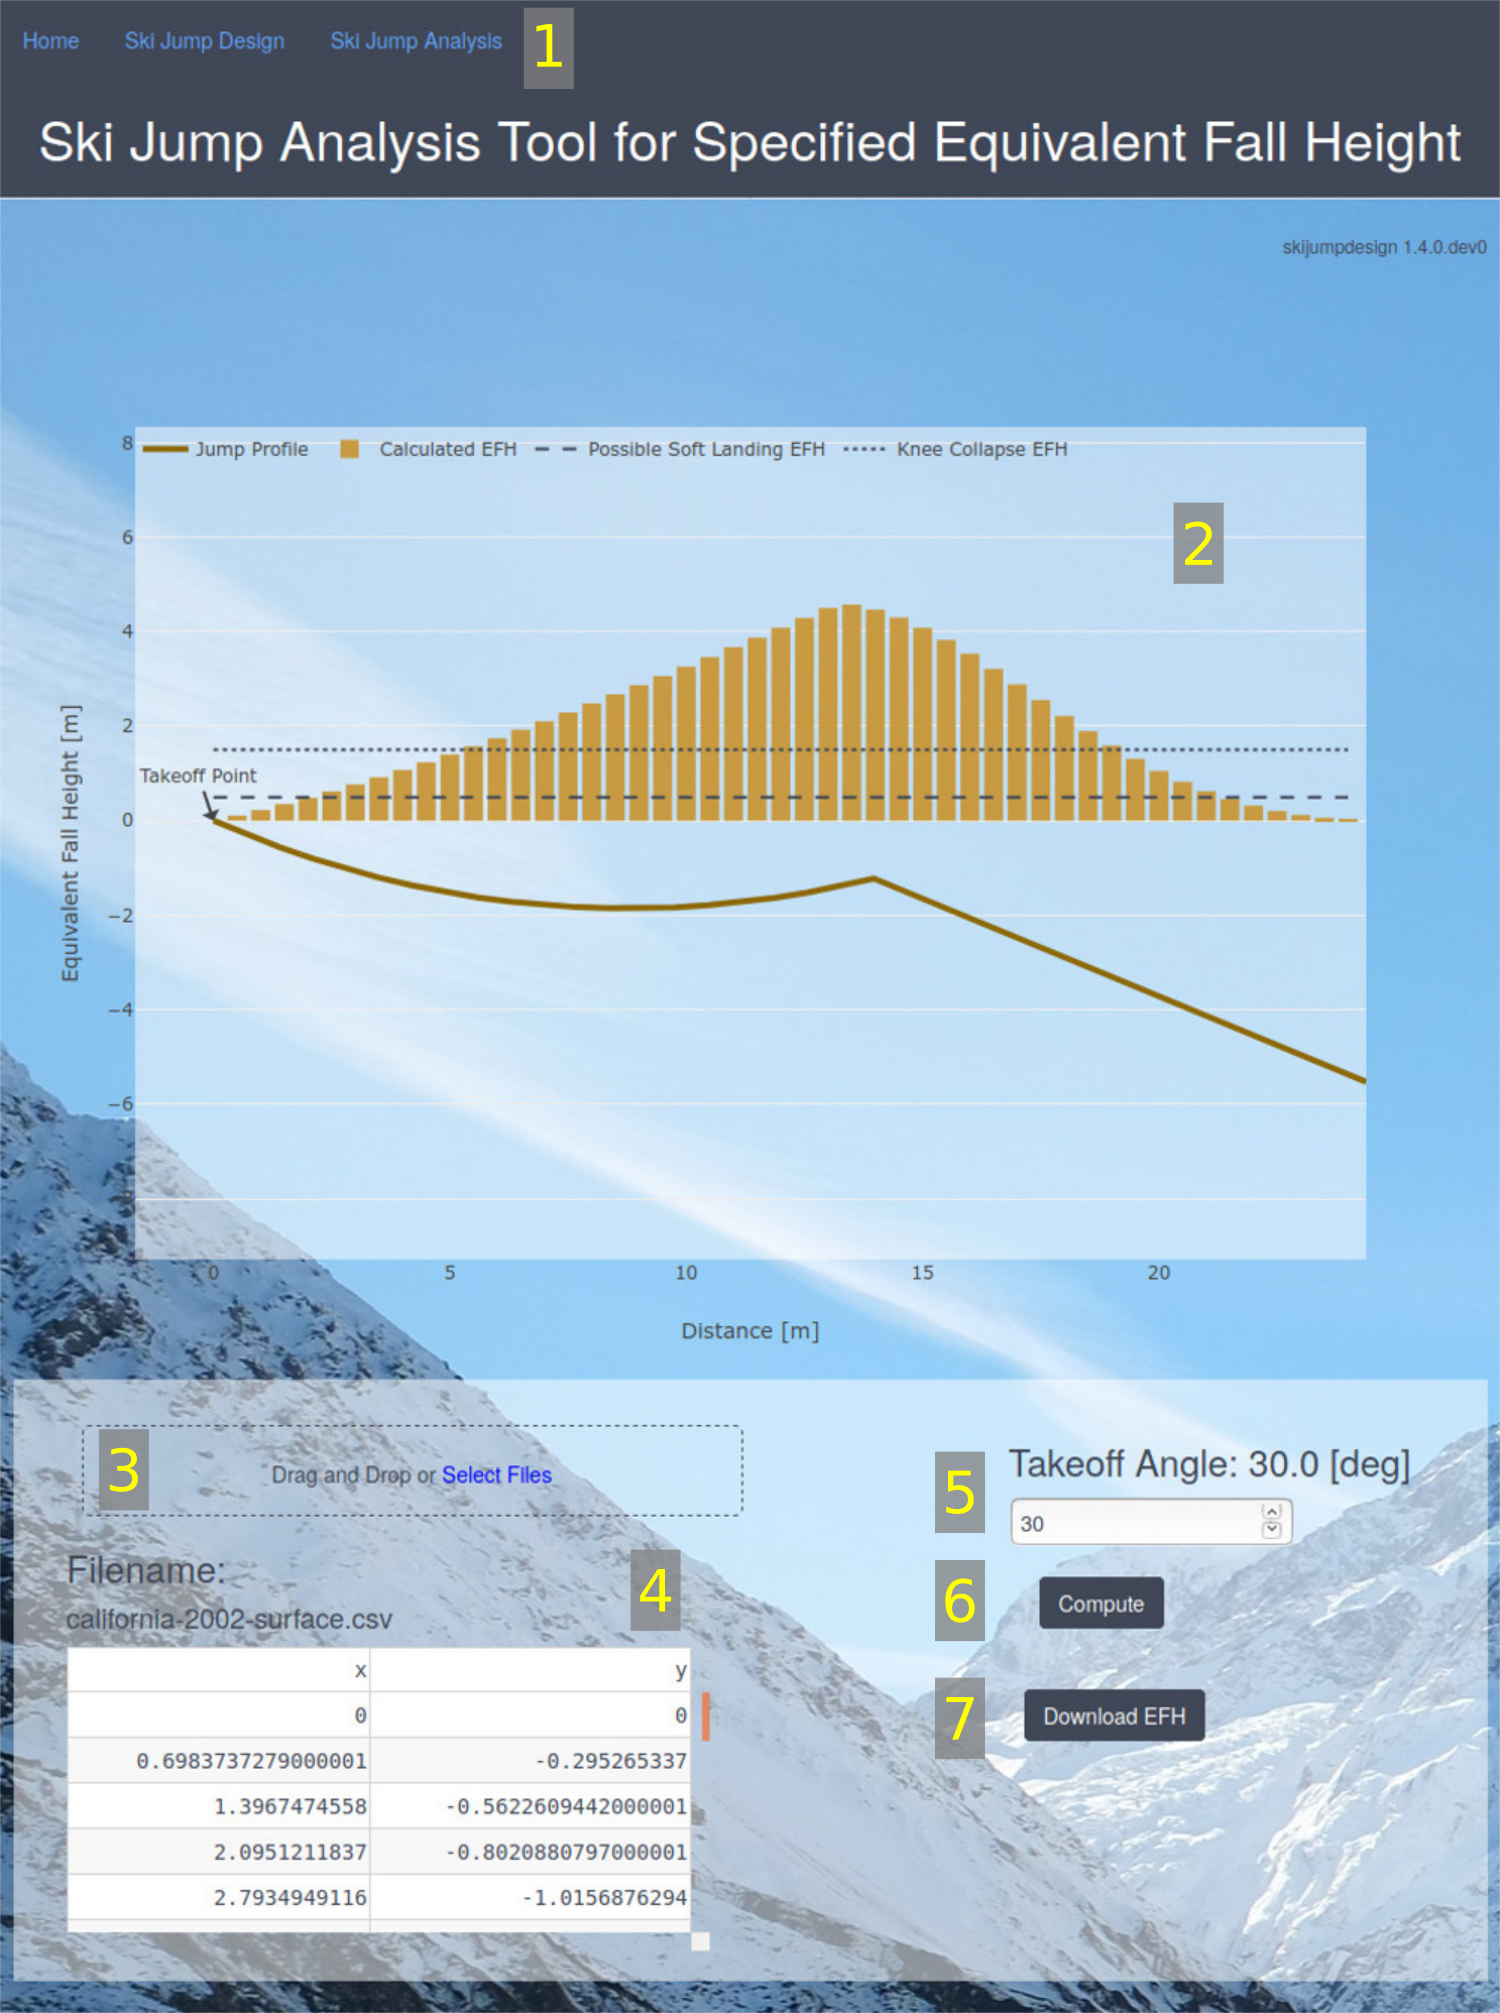
\includegraphics[width=5.00in]{figures/web-app-screenshot.png}
  \caption{\textbf{Screenshot of the web app} The web app consists of the 1)
    menu, 2) interactive plot, 3) file upload widget, 4) file contents display,
    5) takeoff angle input, 4) compute button, and 5) results download button.}
  \label{fig:web-app-screenshot}
\end{figure}

The software is written in Python and uses popular packages including
Cython~\cite{Behnel2011}, matplotlib~\cite{Hunter2007},
NumPy~\cite{Oliphant2006}, pandas~\cite{team2020},
Plotly/Dash~\cite{Inc.2015},pycvodes~\cite{Dalhgren2018},
SciPy~\cite{Virtanen2020}, SymPy~\cite{Meurer2017}, and xlrd.
The software is open source and licensed under the MIT redistribution license.
The source code is available on Gitlab
(\url{https://gitlab.com/moorepants/skijumpdesign}) and PyPi
(\url{https://pypi.org/project/skijumpdesign/}. Users can submit bugs, feature
requests, code improvements, and additions at the Gitlab repository.  The
software is documented at \href{https://skijumpdesign.readthedocs.io}{skijumpdesign.readthedocs.io}.

\section{Jump Shape Measurement}
%
The form of Equation~\ref{eq:efh} requires the Cartesian coordinates and the
slope at each coordinate to compute the equivalent fall height. Direct
measurements of the coordinates can be done with surveying equipment or
accurate GPS tools and indirect measurements can be done less expensively, but
more laboriously.
%
\begin{description}
  \item[Mark the jump center line] Mark a line that defines the projection of
    the jumper's path onto the landing surface. This indicates the cross
    sectional profile that is to be measured.
  \item[Takeoff point] Locate the jumper takeoff point and measure the vertical
    and horizontal location relative to the start of the origin of the tape
    measure.
  \item [Takeoff angle] Measure the absolute slope at the takeoff point using a
    digital level.
  \item[Tape Measure and Level] A flexible tape measure is laid parallel to the
    center line along the surface of the jump. A series of distance
    measurements can be recorded along with the slope at that location. The
    absolute slope can be measured with a digital level. With the distance
    along the curve and the slope at each distance measurement, the Cartesian
    coordinates can be calculated with\todo{describe these calculations or
    reference Mont's ASTM standard}.
\end{description}


\subsection{Surveying}
%
Analog and digital theodolites can be used to measure the relative angles from
the device to points in the distance using standard surveying techniques. The
Carteisan coordinates can be calculated from these measures.

\subsection{Differential GPS}
%
Consumer grade differential GPS units can measure the Cartesian coordinates
directly with 1~\si{\centi\meter} accuracy up to 1~\si{\kilo\meter}
distances from the base station. For example, we have used the 1500 Piksi
differential GPS system (SwiftNav, San Francisco, USA) to record slope shapes
from a roving skier with GPS antenaee mounted to the helmet.

\subsection{Park Profiler}
%
\todo[inline]{Add short description of the park profiler and cite McNeil's
work on it.}

\section{Case Studies}
%
Below we present two case studies derived from cases in the United States in
which the jury ruled in favor of the plaintiffs, in that there was a neglect in
the design and construction of the jumps and that contributed significantly to
the injury severity of the jumpers.
\subsection{Charlene Vine v Bear Valley Ski Company}
%
In 2000, Ms. Charlene Vine's spine was broken on a jump constructed at the Bear Valley
Ski Resort. The jump shape was that of a ``tabletop'' which is a common shape
of ski and snowboarding jumps, but the jump's table, which is normally flat,
was concave. It is the jump constructor's intent that jumpers fully clear the
table when jumping, but Ms. Vine landed short of the end of the table.
Figure~\ref{fig:vine-v-bear-valley} shows a reasonable approximation of the
jump at Bear Valley Ski Resort based on measurements taken of the jump for the
trial.

The lower panel plots the equivalent fall height for different landing
locations. It is clear that short of the table end, that the equivalent fall
height is its highest. Ms. Vine's fall was equivalent to a one to two storey
fall. The green jump profile in the upper panel shows a possible jump design of
similar size with similar possible flight times that ensures a constant
equivalent fall height of 1~\si{\meter}. The average fall heights for 1 and 2
stoery falls are estimated from data in \cite{Vish2005}.
%
\begin{figure}
  \centering
  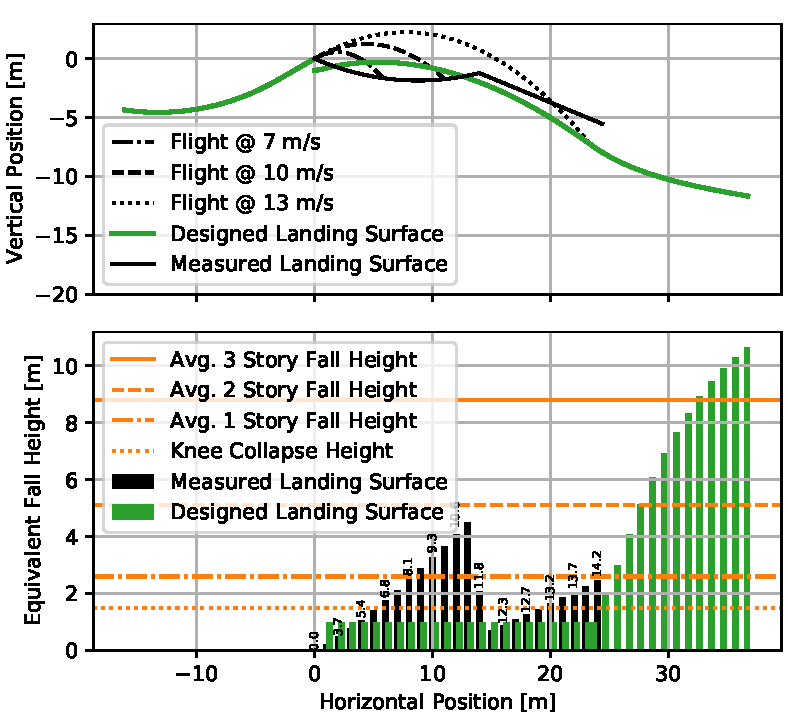
\includegraphics[width=5.25in]{figures/vine-v-bear-valley.pdf}
  \caption{\textbf{Measured Bear Valley ski jump compared to a possible design}}
  \label{fig:vine-v-bear-valley}
\end{figure}

\subsection{Kenny Salvini v Ski Lifts Inc.}
%
\begin{figure}
  \centering
  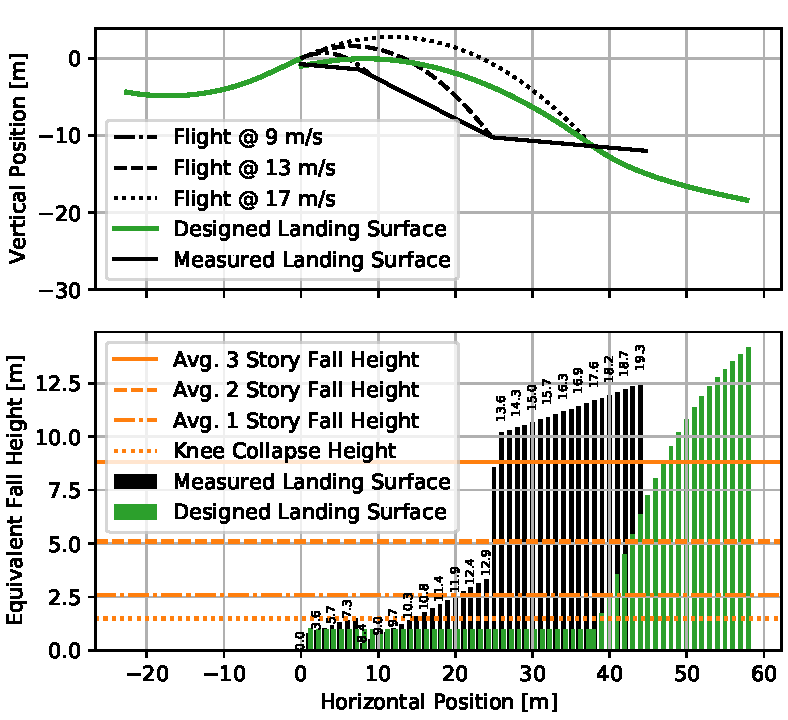
\includegraphics[width=5.25in]{figures/salvini-v-snoqualmie.pdf}
  \caption{\textbf{Measured Snoqualmie ski jump compared to a possible design}}
  \label{fig:salvini-v-snoqualmie}
\end{figure}

\section{Conclusion}
%
\bibliographystyle{plain}
\bibliography{references}

\end{document}
